% ===================================================================
% One Discussion chapter, replacing the former chapters on the hardware
% numbers, the comparison with the baseline, and the discussion.
% ===================================================================
\chapter{Discussion}
\label{ch:discussion}

\section{Which algorithm for a sensor front end?}
\label{sec:choice}

On the same data, lossless prediction matches the best lossy quantiser's ratio
(\num{3.75} against \num{3.76}) at about a third of its missed detections
(Section~\ref{sec:stage1}). Between the two lossless coders, DRHE and LPC are
close on compression ratio, with the leader set by the dictionary, and level on
logic, so the deciding differences lie elsewhere.
DRHE's output depends only on samples already received, so it streams, needs
no frame buffer and lags its input by \SI{13}{\micro\second}. LPC's
coefficients are sums over every ramp of the frame, so its first output bit
must wait for its last input sample, giving \SI{3.0}{\milli\second} of latency
and a \SI{3.0}{\mebi bit} buffer that grows with the frame. This is a property
of the algorithm, not of this implementation. LPC's costs fall on the
compressor: its decoder needs no block RAM, so where a few milliseconds of
latency and the memory are available, its \SI{4}{\percent} better ratio can be
had. A backward-adaptive LPC, fitted to previous frames, would remove the
buffer and the latency at some cost in ratio.

\paragraph{Why DRHE stays in floating point.} Rebuilt with Kiem's fixed-point
types and nothing else changed, the DRHE compressor uses \HW{ablf}{LUT} LUTs and
\HW{ablf}{DSP} DSPs after routing, against \HW{drhen}{LUT} and
\HW{drhen}{DSP}, for a \SI{0.07}{\percent} loss of ratio, so floating point is
not kept for its ratio. It is kept for three reasons. First,
verification: single-precision prediction reproduces the double-precision
MATLAB model's bit counts on every frame, so each level of the ladder can be
checked exactly against the one above, whereas a fixed-point design would need
its own bit-accurate model, which Kiem listed as future work. Agreeing bit counts
do not require identical predictions: where a single- and a double-precision
prediction round to different integers, a residual changes by one, which need
not change its size. A decoder therefore needs the encoder's exact arithmetic,
which is why a double-precision decoder drifts on 8 of the 50 frames whilst the
decoder built from the HLS source is exact (Section~\ref{sec:dechw}). Second,
timing as built: that fixed-point version closes at only \HW{ablf}{fmax}\,MHz,
against \HW{drhen}{fmax}\,MHz for floating point, because its feedback loop, 26
carry-chain levels before the state write, was not re-pipelined. One or two
more pipeline stages would fix this. Third, generality: floating point needs no
word-length analysis for a particular sensor's scaling. On this device the
cost is affordable, since the compressor is \SI{16}{\percent} of the chip; where
silicon area dominates, as in an ASIC, fixed point is the better trade-off.

For a streaming sensor-edge compressor this thesis therefore recommends DRHE:
lossless, \num{4.2} with a matched dictionary, a wide throughput margin, no
frame buffer, and microseconds rather than milliseconds of latency.

\section{Scaling to larger frames}
\label{sec:scaling}

The hardware compresses four of the sixteen receive channels, because four
complex 16-bit samples fill the 128-bit stream. Scaling the measured figures
linearly, all 16 channels would take DRHE about \SI{2.5}{\milli\second} per
frame and LPC about \SI{13}{\milli\second}, with a \SI{12}{\mebi bit} buffer.
Kiem's use case delivers about \SI{3.2}{Gbit/s} of range-FFT codes during
acquisition. DRHE's measured \SI{5.1}{Gbit/s} keeps up without a buffer, but
LPC would take about \SI{69}{\milli\second} per frame, longer than his whole
\SI{50}{\milli\second} cycle, and would need an \SI{8.4}{\mega\byte} frame
buffer against about \SI{4.4}{\mega\byte} of on-chip memory on this device.
DRHE scales with the data rate, whereas LPC scales with the frame size and, on
large frames, runs out of both time and memory.

\section{What the compression ratio measures}
\label{sec:ratiomeaning}

Figure~\ref{fig:bits} follows one value through the compressor. Since the FX16
scale is fixed to a full-scale signal and the largest ColoRadar code is 437,
only $\log_2 437 + 1 = 9.77$ of the 16 bits carry information; removing the
other 6.2 is a factor of \num{1.64}, which any entropy coder achieves. The
sparsity of a range-FFT frame, mostly noise near zero with a few targets, gives
a further \num{2.12}. Prediction then adds \num{1.08} for DRHE and the
re-derived dictionary \num{1.12}.

\begin{figure}[htbp]
\centering
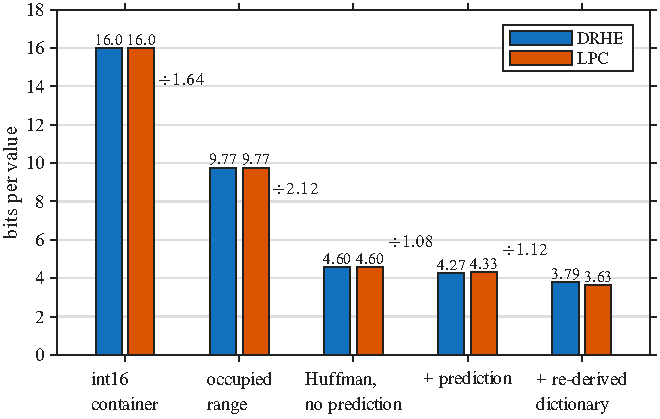
\includegraphics[width=0.8\textwidth]{fig_bits.pdf}
\caption[Where the bits go]{Bits per value through the compressor, 50 frames,
four receive channels. Most of the reduction comes from the unused top of the
16-bit container and from the sparsity of the data, before any prediction.
The first three stages are shared by both algorithms; the factors between
stages are for DRHE.}
\label{fig:bits}
\end{figure}

The ratios are therefore partly a property of the capture. A sensor whose data
filled the container would have no unused bits to remove, and scaled to fill
it the same frame compresses by only \num{1.2} (Section~\ref{sec:quant}).
Ratios from different sensors are only comparable if their gain staging is,
and a no-prediction baseline should be reported with any radar compression
ratio. The unused bits are also why FX16 loses \SI{3.77}{\percent} of the
detections: how many bits of the noise floor are worth transmitting is a choice
for the radar designer, and a lossless compressor only makes that choice
cheaper to carry.

\paragraph{What a different dataset would add.} All of these ratios come from
one indoor recording of a slowly changing scene, captured with gain staging
that leaves six bits of every code unused. A second dataset would show how much
of the result belongs to the methods and how much to this capture. The raw ADC
dataset of Gao \emph{et al.}~\cite{gao2022} is a natural candidate: it was
recorded outdoors on roads, a campus and a parking lot with a TI AWR1843, mostly
with moving pedestrians, cyclists, cars, motorbikes, buses and trucks, and every
object is labelled. It would help in four ways. First, moving targets give
larger Doppler phase steps and more strong returns, a harder test of the
predictors and of a dictionary trained on another scene, so its ratios are
likely to be lower and closer to what a vehicle would see. Second, its gain
staging is different, so reporting its no-prediction baseline beside the
predictive ratios would show directly how much of the ratio comes from unused
headroom rather than from prediction. Third, its labels would allow detection
losses to be counted on real objects rather than on range--Doppler cells.
Fourth, its radar time-multiplexes two transmitters, so it would test the
prediction-lag result at $\nTx = 2$. Its array is far smaller, 8 virtual
channels against ColoRadar's 192, so it produces far less data per frame; it
would complement the cascade data used here rather than replace it.

\section{Threats to validity}
\label{sec:threats}

\begin{itemize}
\item All results use 50 frames of one indoor recording, and much of the ratio
comes from its gain staging (Section~\ref{sec:ratiomeaning}). Busier scenes
would give lower ratios, and the dictionaries were trained and tested on the
same recording.
\item The lag $\nTx$ is specific to TDM; Doppler- or code-division MIMO has no
interleaved ramp axis.
\item The detection chain is simpler than a production one (no angle FFT, a
Doppler FFT across all 192 ramps in their transmitter-interleaved order, no
positional tolerance, a fixed threshold), so the lossy schemes' rates should be
read as relative. BAQ is represented by a block-floating-point quantiser.
\item Stage~1 uses 16 receive channels and the hardware four, and power is a
Vivado estimate, not a measurement.
\end{itemize}
